%%%%%%%%%%%%%%%%%%%%%%%%%%%%%%%%%%%%%%%%%%%%%%%%%%%%%%%%%%%%%%%%%%%%%%%%%%%%%%%%%%%%%%%%%%%%%%%%%%%%%%%%%%%%%%%%%%%%%%%%%%%%%%%%%%%%%%%%%%%%%%%%%%%%%%%%%%%%%%%%%%%%%%%%%%%%%%%%%%%%%%%%%%%%
% Written By Michael Brodskiy
% Class: Linear Algebra
% Professor: L. Knight
%%%%%%%%%%%%%%%%%%%%%%%%%%%%%%%%%%%%%%%%%%%%%%%%%%%%%%%%%%%%%%%%%%%%%%%%%%%%%%%%%%%%%%%%%%%%%%%%%%%%%%%%%%%%%%%%%%%%%%%%%%%%%%%%%%%%%%%%%%%%%%%%%%%%%%%%%%%%%%%%%%%%%%%%%%%%%%%%%%%%%%%%%%%%

\documentclass[12pt]{article} 
\usepackage{alphalph}
\usepackage[utf8]{inputenc}
\usepackage[russian,english]{babel}
\usepackage{titling}
\usepackage{amsmath}
\usepackage{graphicx}
\usepackage{enumitem}
\usepackage{amssymb}
\usepackage{physics}
\usepackage{tikz}
\usepackage{mathdots}
\usepackage{yhmath}
\usepackage{cancel}
\usepackage{color}
\usepackage{siunitx}
\usepackage{array}
\usepackage{multirow}
\usepackage{gensymb}
\usepackage{tabularx}
\usepackage{booktabs}
\usetikzlibrary{fadings}
\usetikzlibrary{patterns}
\usetikzlibrary{shadows.blur}
\usetikzlibrary{shapes}
\usepackage[super]{nth}
\usepackage{expl3}
\usepackage[version=4]{mhchem}
\usepackage{hpstatement}
\usepackage{rsphrase}
\usepackage{everysel}
\usepackage{ragged2e}
\usepackage{geometry}
\usepackage{fancyhdr}
\usepackage{cancel}
\usepackage{multicol}
\geometry{top=1.0in,bottom=1.0in,left=1.0in,right=1.0in}
\newcommand{\subtitle}[1]{%
  \posttitle{%
    \par\end{center}
    \begin{center}\large#1\end{center}
    \vskip0.5em}%

}
\usepackage{hyperref}
\hypersetup{
colorlinks=true,
linkcolor=blue,
filecolor=magenta,      
urlcolor=blue,
citecolor=blue,
}

\urlstyle{same}


\title{Linear Algebra 1.1 Homework}
\date{}
\author{Michael Brodskiy\\ \small Instructor: Prof. Knight}

% Mathematical Operations:

% Sum: $$\sum_{n=a}^{b} f(x) $$
% Integral: $$\int_{lower}^{upper} f(x) dx$$
% Limit: $$\lim_{x\to\infty} f(x)$$

\begin{document}

\maketitle

\begin{enumerate}

    \setcounter{enumi}{2}

  \item Not linear

    \setcounter{enumi}{4}

  \item Not linear

    \setcounter{enumi}{8}

  \item 

    \begin{equation*}
      \begin{split}
        y&\rightarrow s\\
        z&\rightarrow t\\
        S&=\left\{ (1-s-t,s,t) \right\}
      \end{split}
      \label{1}
    \end{equation}

  \item

    \begin{equation*}
      \begin{split}
        x_2&\rightarrow s\\
        x_3&\rightarrow t\\
        S&=\left\{ (1-2s+3t,s,t) \right\}
      \end{split}
      \label{2}
    \end{equation}

  \item \textbf{ }

    \begin{multicols}{2}

      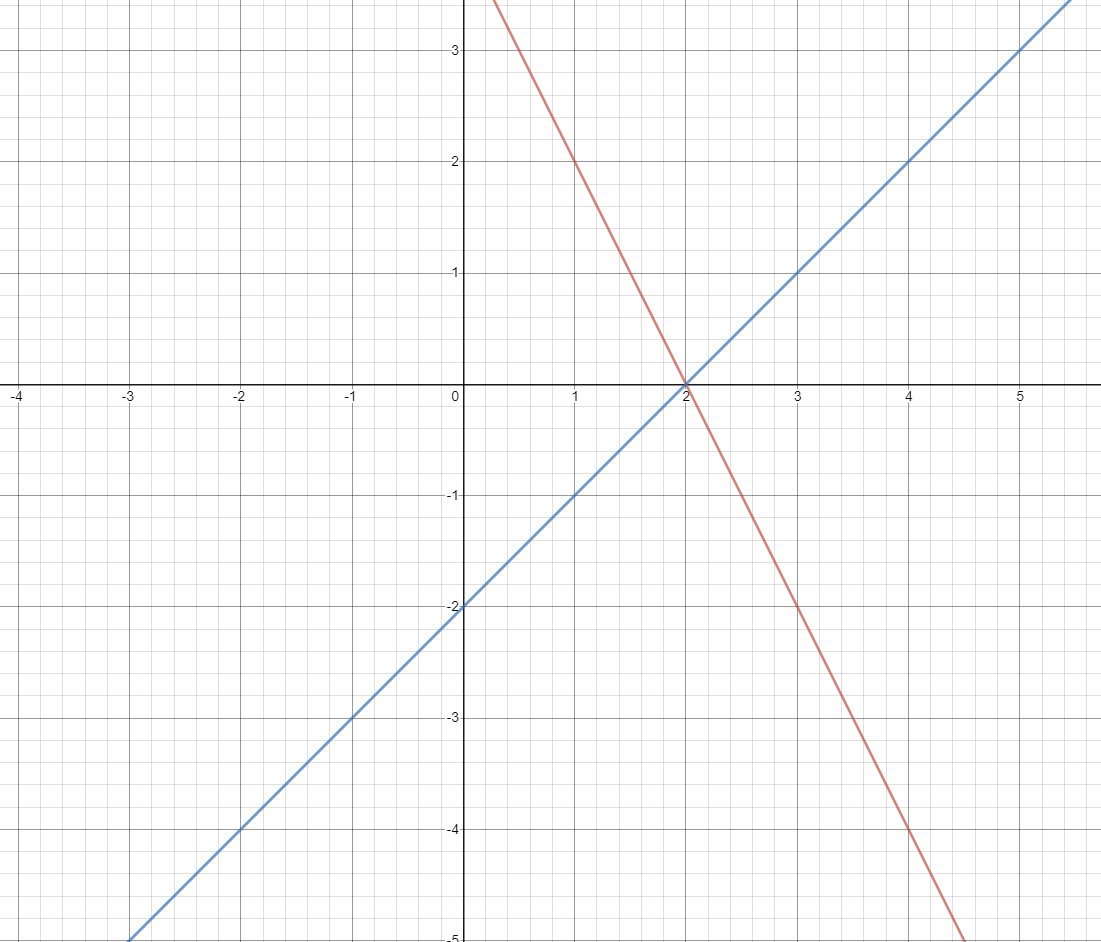
\includegraphics[width=.5\textwidth]{../Figures/Prob11Graph.png}

    \begin{equation*}
      \begin{split}
        \begin{array}{l l}
          2x+y=4 & L_1\\
          x-y=2 & L_2
        \end{array}\\
        L_1-L_2\rightarrow x=2\\
        2(2)+y=4\\
        y=0\\
        \text{The solution is at point } (2,0)
      \end{split}
      \label{3}
    \end{equation}

  \end{multicols}

    \setcounter{enumi}{12}

  \item \textbf{ }

    \begin{multicols}{2}

      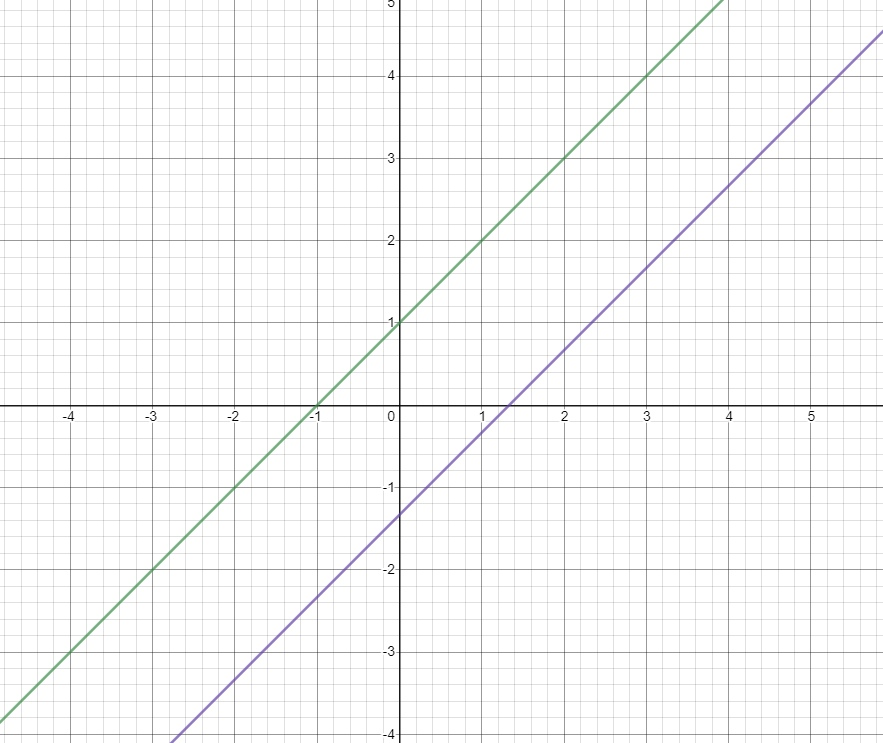
\includegraphics[width=.5\textwidth]{../Figures/Prob13Graph.png}

    \begin{equation*}
      \begin{split}
        \begin{array}{l l}
          -x+y=1 & L_1\\
          3x-3y=4 & L_2
        \end{array}\\
        -\frac{1}{3}L_2\rightarrow -x+y=-\frac{4}{3}\\
        \text{No Solution, Lines Parallel}
      \end{split}
      \label{4}
    \end{equation}

  \end{multicols}

    \setcounter{enumi}{14}

  \item \textbf{ }

    \begin{multicols}{2}

      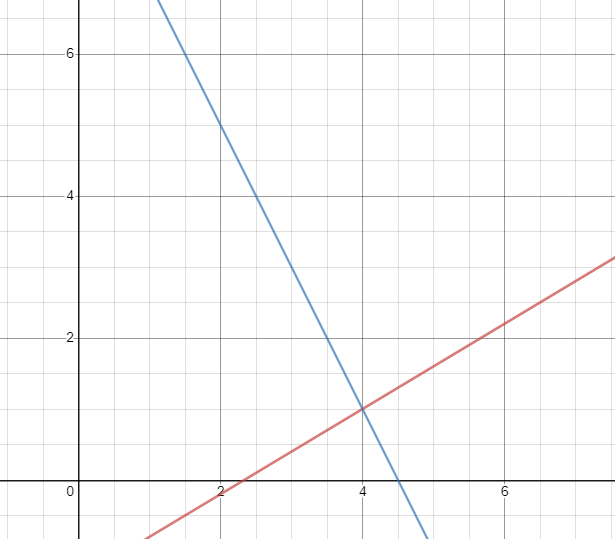
\includegraphics[width=.5\textwidth]{../Figures/Prob15Graph.png}

    \begin{equation*}
      \begin{split}
        \begin{array}{l l}
          3x-5y=7 & L_1\\
          2x+y=9 & L_2
        \end{array}\\
        5L_2+L_1\rightarrow 13x=52\\
        x=4\\
        2(4)+y=9\\
        y=1\\
        \text{The solution is at point } (4,1)
      \end{split}
      \label{5}
    \end{equation}

  \end{multicols}

  \newpage

    \setcounter{enumi}{16}

  \item \textbf{ }

    \begin{multicols}{2}

      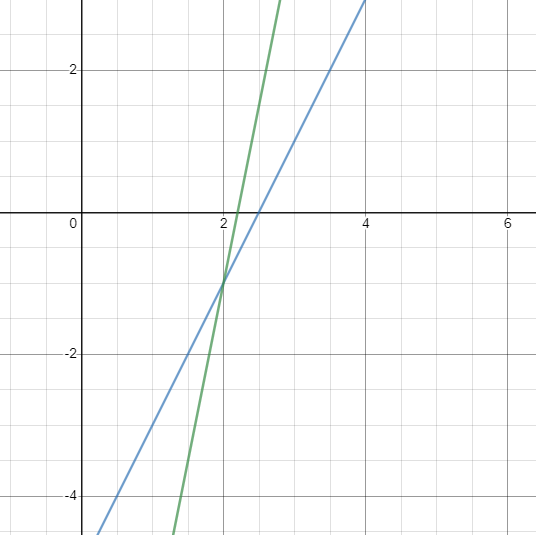
\includegraphics[width=.5\textwidth]{../Figures/Prob17Graph.png}

    \begin{equation*}
      \begin{split}
        \begin{array}{l l}
          2x-y=5 & L_1\\
          5x-y=11 & L_2
        \end{array}\\
        L_2-L_1\rightarrow 3x=6\\
        x=2\\
        2(2)-y=5\\
        y=-1\\
        \text{The solution is at point } (2,-1)
      \end{split}
      \label{6}
    \end{equation}

  \end{multicols}

    \setcounter{enumi}{18}

  \item \textbf{ }

    \begin{multicols}{2}

      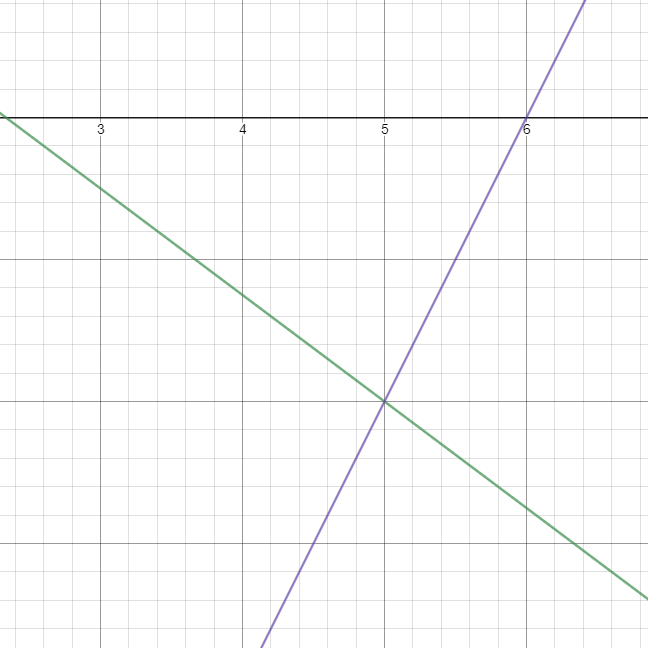
\includegraphics[width=.5\textwidth]{../Figures/Prob19Graph.png}

    \begin{equation*}
      \begin{split}
        \begin{array}{l l}
          \frac{x+3}{4}+\frac{y-1}{3}=1 & L_1\\
          2x-y=12 & L_2
        \end{array}\\
        12L_1\rightarrow 3x+4y=7\\
        4L_2+(3x+4y=7)\rightarrow 11x=55\\
        x=5\\
        2(5)-y=12\\
        y=-2\\
        \text{The solution is at point } (5,-2)
      \end{split}
      \label{7}
    \end{equation}

  \end{multicols}

  \newpage

    \setcounter{enumi}{20}

  \item \textbf{ }

    \begin{multicols}{2}

      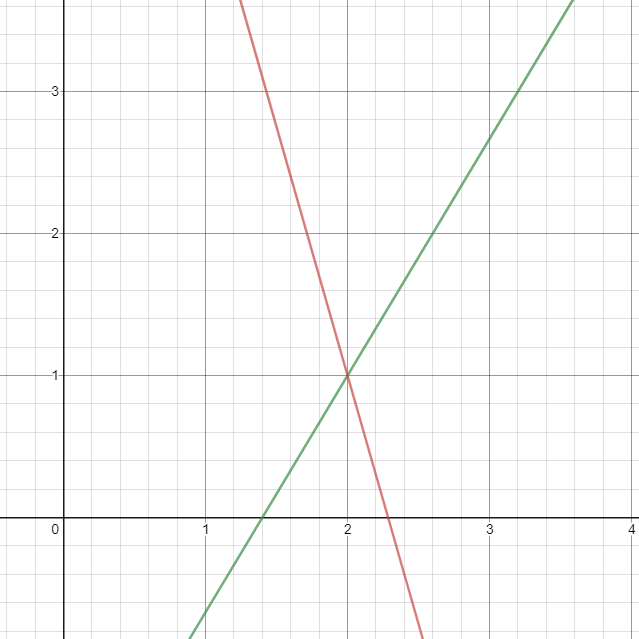
\includegraphics[width=.5\textwidth]{../Figures/Prob21Graph.png}

    \begin{equation*}
      \begin{split}
        \begin{array}{l l}
          .05x-.03y=.07 & L_1\\
          .07x+.02y=.16 & L_2
        \end{array}\\
        200L_1+300L_2\rightarrow 31x=62\\
        x=2\\
        .05(2)-.03y=.07\\
        y=1\\
        \text{The solution is at point } (2,1)
      \end{split}
      \label{8}
    \end{equation}

  \end{multicols}

    \setcounter{enumi}{22}

  \item \textbf{ }

    \begin{multicols}{2}

      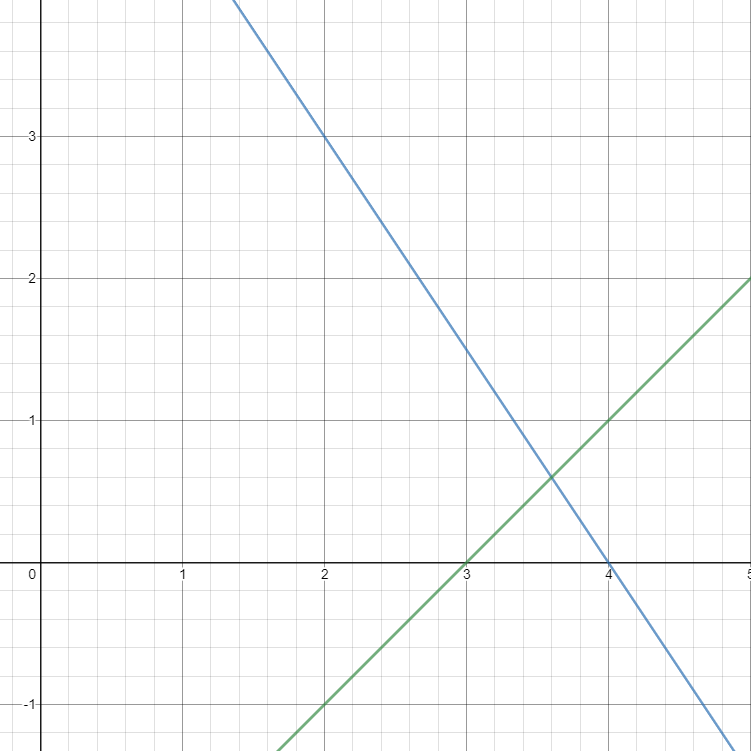
\includegraphics[width=.5\textwidth]{../Figures/Prob23Graph.png}

    \begin{equation*}
      \begin{split}
        \begin{array}{l l}
          \frac{x}{4} + \frac{y}{6} = 1 & L_1\\
          x-y=3 & L_2
        \end{array}\\
        24L_1\rightarrow 6x+4y=24\\
        4L_2+(6x+4y=24)\rightarrow 10x=36\\
        x=3.6\\
        -y=3-3.6\\
        y=.6\\
        \text{The solution is at point } (3.6,0.6)
      \end{split}
      \label{9}
    \end{equation}

  \end{multicols}

    \setcounter{enumi}{24}

  \item $\begin{array}{|r|} \hline x_1-x_2=2\\ x_2=3\\ \hline \end{array} \rightarrow x_1=2+3 \rightarrow x_1=5$

    \begin{equation*}
      S=\left\{ (5,3) \right\}
      \label{10}
    \end{equation}

    \setcounter{enumi}{26}

  \item $\begin{array}{|r|} \hline -x+y-z=0\\ 2y+z=3\\ \frac{1}{2}z=0\\ \hline\end{array} \rightarrow z=0 \rightarrow 2y=3 \rightarrow y=\frac{3}{2} \rightarrow -x=-\frac{3}{2}\rightarrow x=\frac{3}{2}$

    \begin{equation*}
      S=\left\{ \frac{3}{2},\frac{3}{2},0 \right\}
      \label{11}
    \end{equation}

    \setcounter{enumi}{28}

  \item $\begin{array}{|r|} \hline 5x_1 + 2x_2 + x_3 = 0\\ 2x_1+x_2=0\\ \hline\end{array} \rightarrow x_1=-\frac{x_2}{2} \rightarrow x_3 = t \rightarrow x_2 = 2t \rightarrow x_3 = -t  $ 

    \begin{equation*}
      S=\left\{ -t,2t,t \right\}
      \label{12}
    \end{equation}

    \setcounter{enumi}{38}

  \item

    \begin{equation*}
      \begin{split}
        \begin{array}{l l}
          3u + v = 240 & L_1\\
          u + 3v = 240 & L_2
        \end{array}\\
        3L_2 - L_1\rightarrow 8v=480\\
        v=60\\
        u=\frac{240-60}{3}\\
        u=60\\
        \text{The solution is at point } (60,60)
      \end{split}
      \label{13}
    \end{equation}

    \setcounter{enumi}{40}

  \item

    \begin{equation*}
      \begin{split}
        \begin{array}{l l}
          9x-3y=-1 & L_1\\
          \frac{1}{5}x + \frac{2}{5}y = -\frac{1}{3} & L_2
        \end{array}\\
        45L_2 - L_1\rightarrow 21y=-14\\
        y=-\frac{2}{3}\\
        9x+2=-1\\
        x=-\frac{1}{3}\\
        \text{The solution is at point } \left( -\frac{1}{3},-\frac{2}{3} \right)
      \end{split}
      \label{14}
    \end{equation}

    \setcounter{enumi}{46}

  \item

    \begin{equation*}
      \begin{split}
        \begin{array}{l l}
          x-y-z=0 & L_1\\
          x+2y-z=6 & L_2\\
          2x-z=5 & L_3
        \end{array}\\
        x-z=y\\
        2y+y=6\rightarrow y=2\\
        \begin{array}{l l}
          x-z=2  & L_4\\
          2x-z=5 & L_5
        \end{array}\\
        L_5-L_4\rightarrow x=3\\
        z=1\\
        \text{The solution is at point } \left( 3,2,1 \right)
      \end{split}
      \label{15}
    \end{equation}


    \setcounter{enumi}{48}

  \item 

    \begin{equation*}
      \begin{split}
        \begin{array}{l l}
          3x_1-2x_2+4x_3=1 & L_1\\
          x_1+x_2-2x_3=3 & L_2\\
          2x_1-3x_2+6x_3=8 & L_3
        \end{array}\\
        \text{No solution, planes parallel}
      \end{split}
      \label{16}
    \end{equation}

    \setcounter{enumi}{50}

  \item

    \begin{equation*}
      \begin{split}
        \begin{array}{l l}
          2x_1+x_2-3x_3=4 & L_1\\
          4x_1+2x_3=10 & L_2\\
          -2x_1+3x_2-13x_3=-8 & L_3
        \end{array}\\
        L_3-3L_1+2L_2\rightarrow -18x_3=0\\
        x_3=t\\
        4x_1+2t=10\\
        x_1=\frac{5-t}{2}\\
        5-t+x_2-3t=4\\
        x_2=4t-1\\
        \text{The solution is at } \left( \frac{5-t}{2},4t-1,t \right)
      \end{split}
      \label{51}
    \end{equation}

    \setcounter{enumi}{52}

  \item

    \begin{equation*}
      \begin{split}
        \begin{array}{l l}
          x-3y+2z=18 & L_1\\
          5x-15y+10z=18 & L_2
        \end{array}\\
        \text{No solution, planes parallel}
      \end{split}
      \label{18}
    \end{equation}


    \setcounter{enumi}{64}

  \item The system must have at least one solution because the number of rows is equal to the number of unknowns, and the lines are distinctly different (not parallel). Also, because it is a homogeneous system, $x$, $y$, and $z$ equaling zero can always be a solution.

    \begin{equation*}
      \begin{split}
        \begin{array}{l l}
          5x+5y-z=0 & L_1\\
          10x+5y+2z=0 & L_2\\
          5x+15y-9z=0 & L_3
        \end{array}\\
        L_2-L_1=5x+3z=0\\
        L_3-L_1=10y-8z=0\\
        z=t\\
        y=\frac{4}{5}t\\
        x=-\frac{3}{5}t\\
        \text{The solution is } \left( -\frac{3}{5}t,\frac{4}{5}t,t \right)
      \end{split}
      \label{19}
    \end{equation}

    \setcounter{enumi}{68}

  \item 

    \begin{enumerate}

      \item This is true because it can always be represented as a dependent, parametrized system.

      \item This is false because the planes could be parallel

      \item This is false because a consistent system may only have a single solution

    \end{enumerate}

    \setcounter{enumi}{70}

  \item One such system is the single equation: $x_1-\frac{x_2}{3}=\frac{4}{3}$. If $x_1=t$, then $\frac{x_2}{3}=-\frac{4}{3}+t\rightarrow x_2=3t-4$. Additionally, if $x_2=t$, then $x_1=\frac{x_2+4}{3}$.

    \setcounter{enumi}{74}

  \item

    \begin{equation*}
      \begin{split}
        \begin{array}{l l}
          2A+B-3C=4 & L_1\\
          4A+2C=10 & L_2\\
          -2A+3B-13C=-8 & L_3
        \end{array}\\
        \text{Same as \eqref{51}}\\
        A=\frac{5-t}{2}\\
        B=4t-1\\
        C=t\\
        \text{This means: }\\
        x=\frac{2}{5-t}\\
        y=\frac{1}{4t-1}\\
        z=\frac{1}{t}
        \text{Where }t\neq\frac{1}{4},5,0
      \end{split}
      \label{20}
    \end{equation}

    \setcounter{enumi}{76}

  \item

    \begin{equation*}
      \begin{split}
        \begin{array}{l l}
          (\cos \theta)x + (\sin \theta) y = 1 & L_1\\
          (-\sin \theta)x + (\cos \theta) y = 0 & L_2\\
          x=\frac{\cos\theta}{\sin\theta}y\\
          (\cos^2\theta)y+(\sin^2\theta)y=\sin\theta\\
          (\cos^2\theta+\sin^2\theta)y=\sin\theta\\
          y=\sin\theta\\
          (\cos\theta)x+(\sin^2\theta)=1\\
          x=\cos\theta\\
          \text{The solution is }\left( \cos\theta,\sin\theta \right)
        \end{array}\\
      \end{split}
      \label{21}
    \end{equation}

    \setcounter{enumi}{78}

  \item For no solution, systems must be parallel

    \begin{equation}
      \begin{split}
        \begin{array}{l l}
          x + ky = 2 & L_1\\
          kx+y=4 & L_2
          \end{array}\\
          L_1-\frac{1}{k}L_2\rightarrow \left( k-\frac{1}{k} \right)y=2-\frac{4}{k}\\
          \left( k^2-1 \right)y=2k-4\\
          \text{The statement is not possible for }k=\pm1
      \end{split}
      \label{22}
    \end{equation}

    \setcounter{enumi}{80}

  \item Any $n$ x $n$ system has exactly one solution. This means that, as long as $k\neq0$, the statement is true

    \setcounter{enumi}{82}

  \item Lines must be equal to each other to have infinite solutions

    \begin{equation}
      \begin{split}
        \begin{array}{l l}
          4x + ky = 6 & L_1\\
          kx+y=-3 & L_2
          \end{array}\\
          -2L_2\rightarrow -2kx-2y=6\\
          4x+ky=-2kx-2y\\
          k=-2
      \end{split}
      \label{23}
    \end{equation}

    \setcounter{enumi}{84}

  \item It is not possible to find a solution when $k=1$ because the planes are all parallel. Additionally, the same holds true for $k=-2$, because it is then not possible to solve the system.

\end{enumerate}

\end{document}

